% MWE of generating a slope field of a differential equation
% with a calculated solution given an initial value
% written by
% <erik@heckman.ca> erik ben heckman  2021-03-22
% informed by
% https://tex.stackexchange.com/a/471743 (CC BY-SA 4.0)
% and
% https://tex.stackexchange.com/a/471720 (CC BY-SA 3.0)

\documentclass[border=5pt,tikz]{standalone}
\usepackage[]{tkz-defield}


\begin{document}

\begin{tikzpicture} [
declare function={f(\x,\y)=(1-\x)*\y-\x^2;},
]
\defield[title={\( y'=(1-x)y-x^2\)},]
\end{tikzpicture}

\begin{tikzpicture} [
declare function={g(\x,\y)=(1-\x)*\y^2-\x^2;}
]

\defield[title={\( y'=(1-x)y^2-x^2\)},function=g,no axes][
% \tkzAxeXY
\tkzGrid
]
\end{tikzpicture}

\end{document}

